% !Mode:: "TeX:UTF-8"

\chapter{开发流程}

\section{小组分工}

小组开发采用严格的前后端分离开发模式,前后端分别由不同的组员进行编写并分别测试,每当一个阶段整体完成之后,再做统一的集成测试。

下面是组内成员的具体分工:

\subsection*{周圣喻}主要负责前端部分。负责饿了么前端界面、VUE前端代码编写以及新功能前端的开发。

\subsection*{梁益铭}主要负责后端部分和项目测试。负责JDBC项目,Servlet和Springboot项目的编写、前后端连接测试以及新功能后端的开发。

\subsection*{郑志嘉}主要负责后端部分和数据库连接。负责JDBC项目,Servlet和Springboot项目的编写以及数据库连接管理。
~\\
\section{代码仓库}

小组使用github进行远程仓库管理,再结合git实现项目的合作编写,每个人完成自己的部分后,首先将远程仓库的代码拉取到本地仓库,解决冲突后再将修改后的代码推送到github上,完成一整个阶段后再统一做集成测试。

仓库分为两个分支,main分支存储的是课程项目的部分,advance分支存储的是新功能开放的过程,整个项目小组总共提交了上百次,下面是github上的一些统计数据:

\begin{figure}[H]
    \centering
    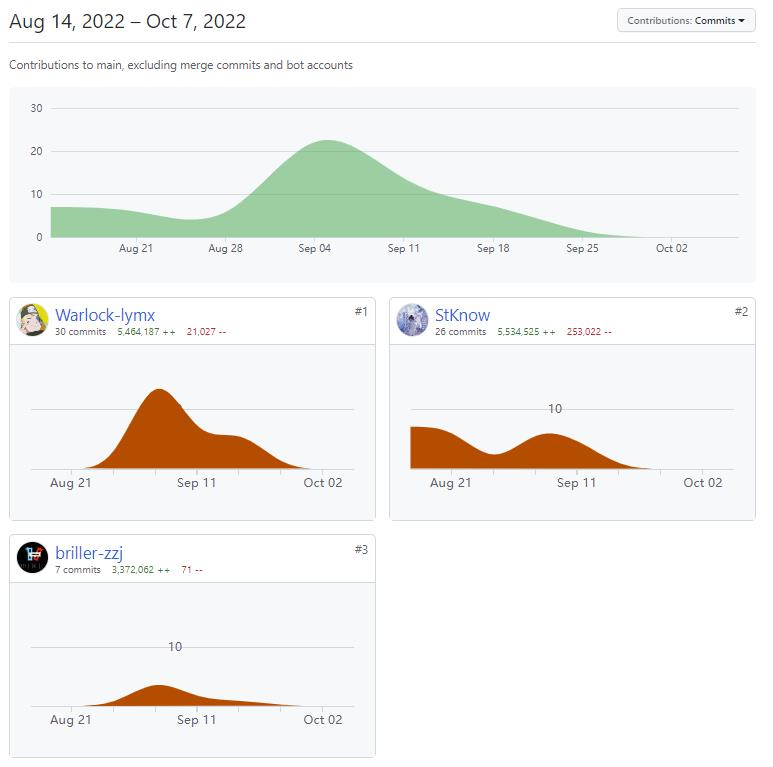
\includegraphics[scale=0.7]{figures/6.1.1.png}
    \caption{提交记录}
\end{figure}

\begin{figure}[H]
    \centering
    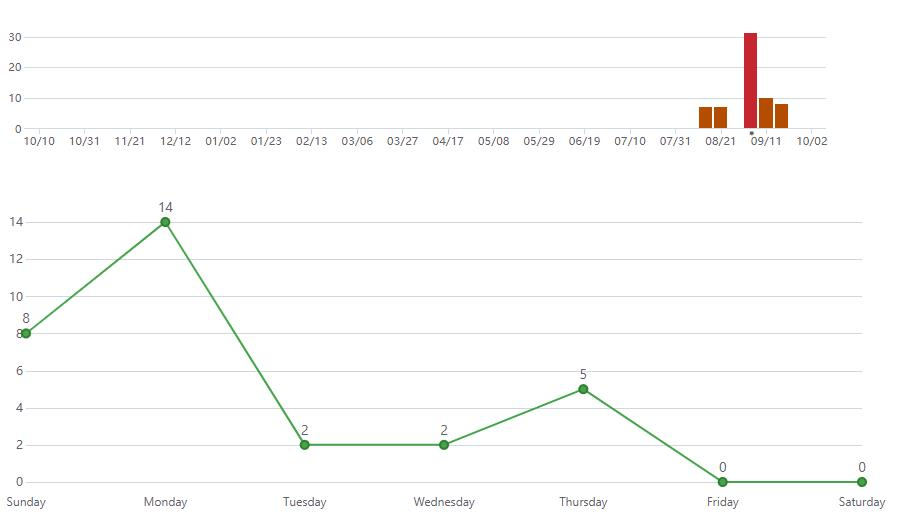
\includegraphics[scale=0.7]{figures/6.1.2.png}
    \caption{提交统计}
\end{figure}

\subsection{实现结果}
\begin{figure}[H]
    \centering
    \subfigure{
        \begin{minipage}[t]{0.48\linewidth}
            \centering
            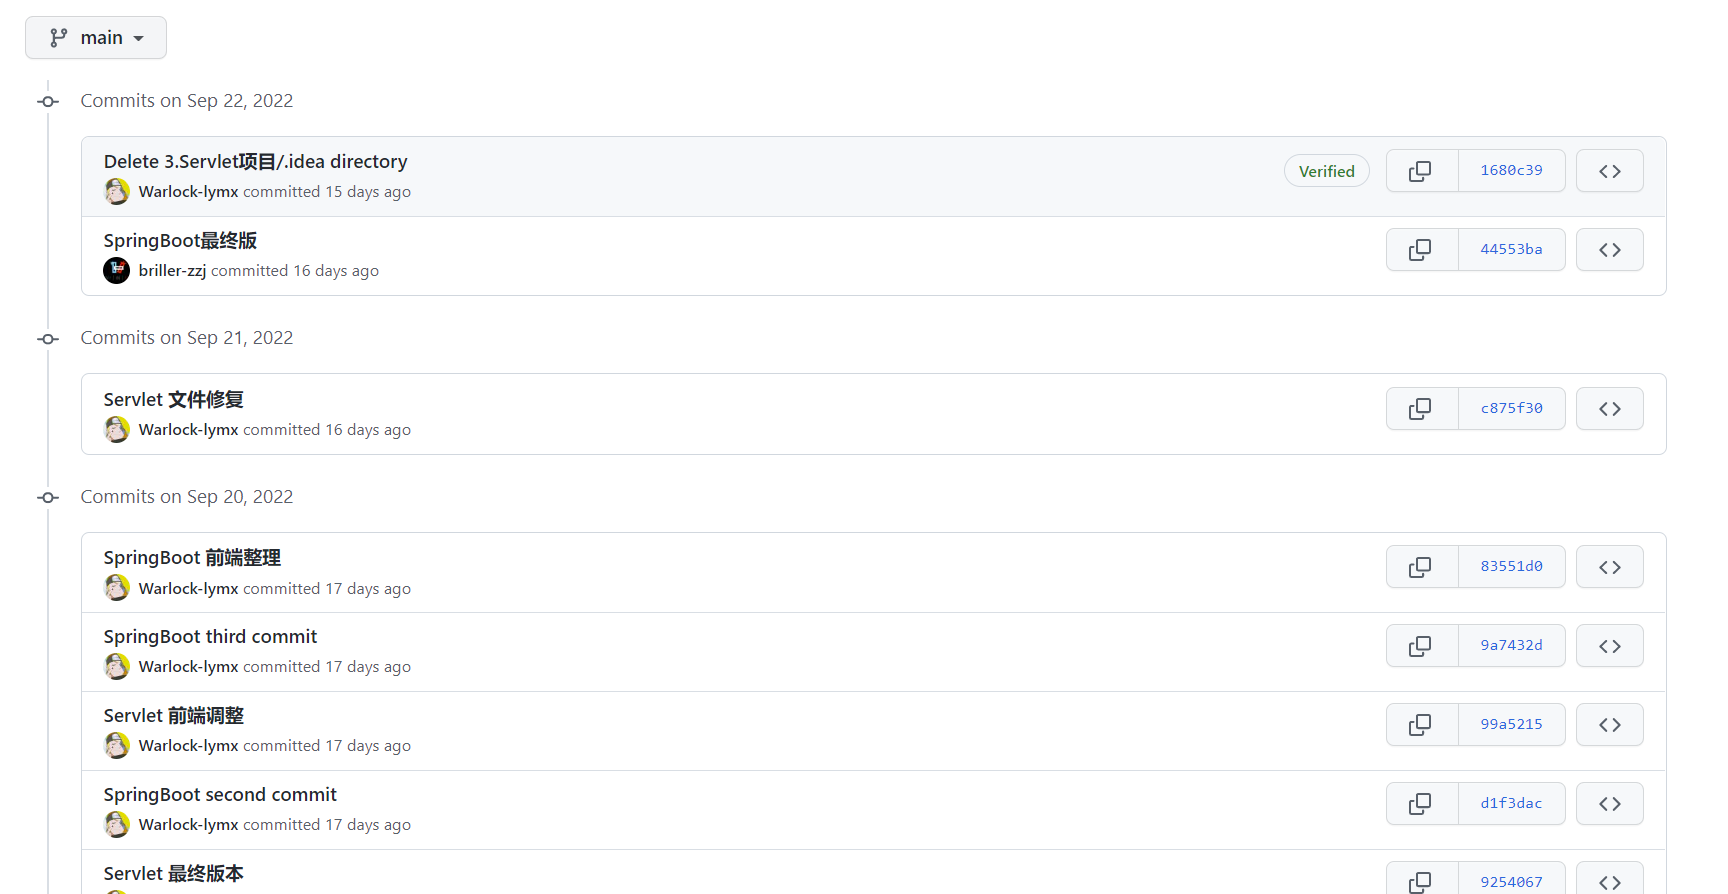
\includegraphics[width=6cm,height=4cm]{figures/6.1.3.png}\\
        \end{minipage}
    }
    \subfigure{
        \begin{minipage}[t]{0.48\linewidth}
            \centering
            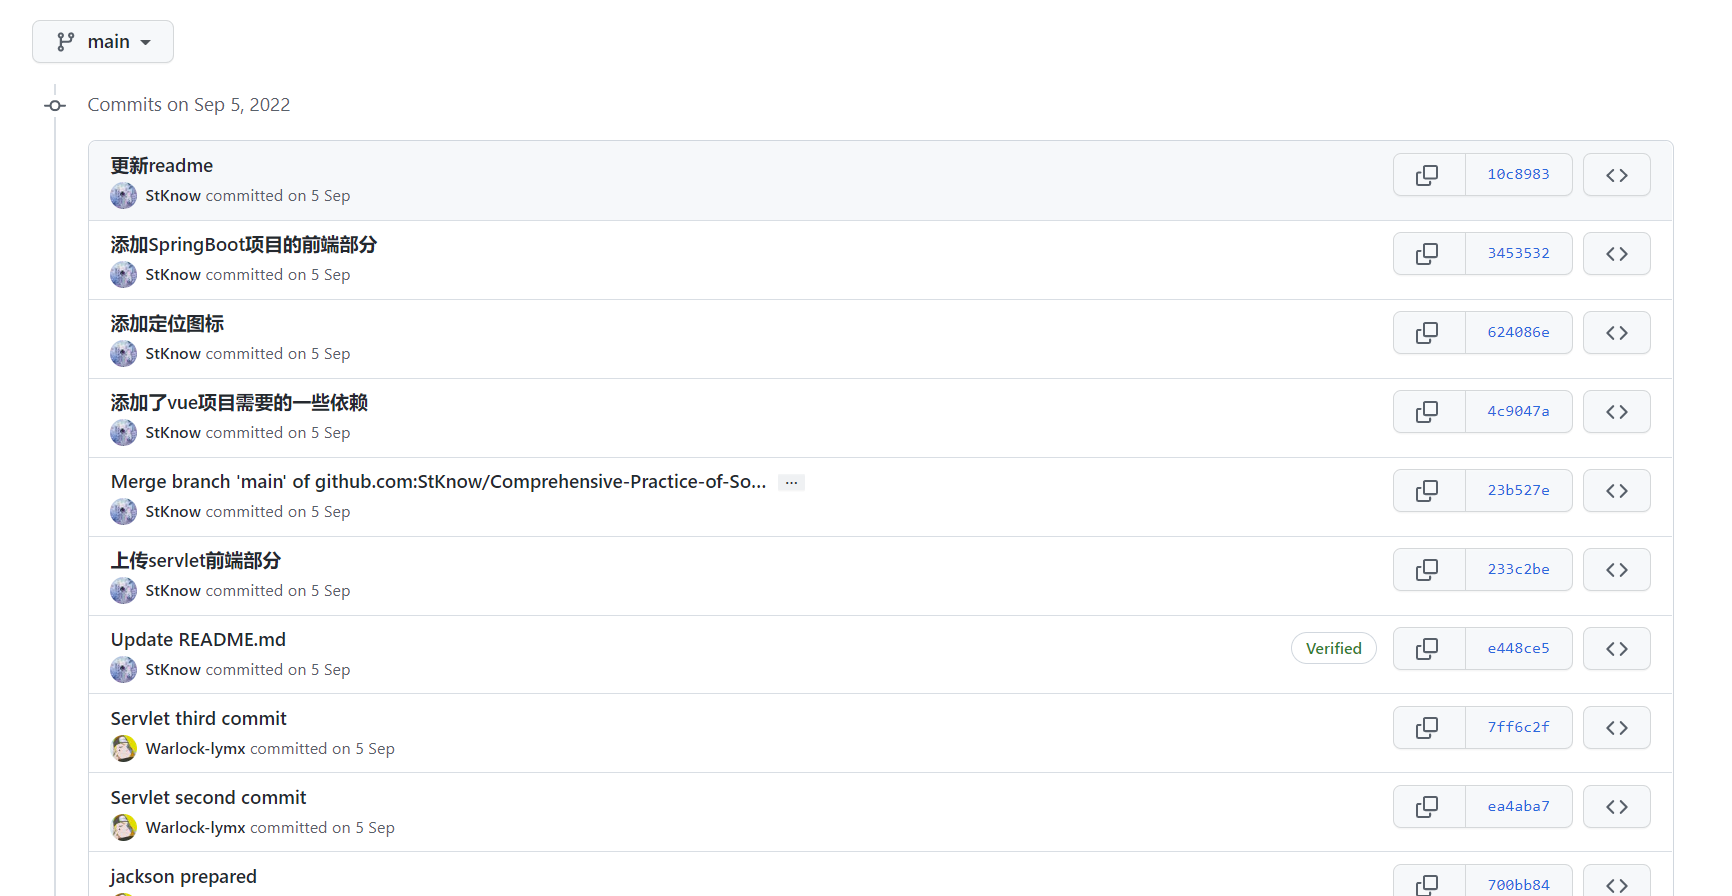
\includegraphics[width=6cm,height=4cm]{figures/6.1.4.png}\\
        \end{minipage}
    }
    \centering
    \caption{main分支提交记录}
\end{figure}

\begin{figure}[H]
    \centering
    \subfigure{
        \begin{minipage}[t]{0.48\linewidth}
            \centering
            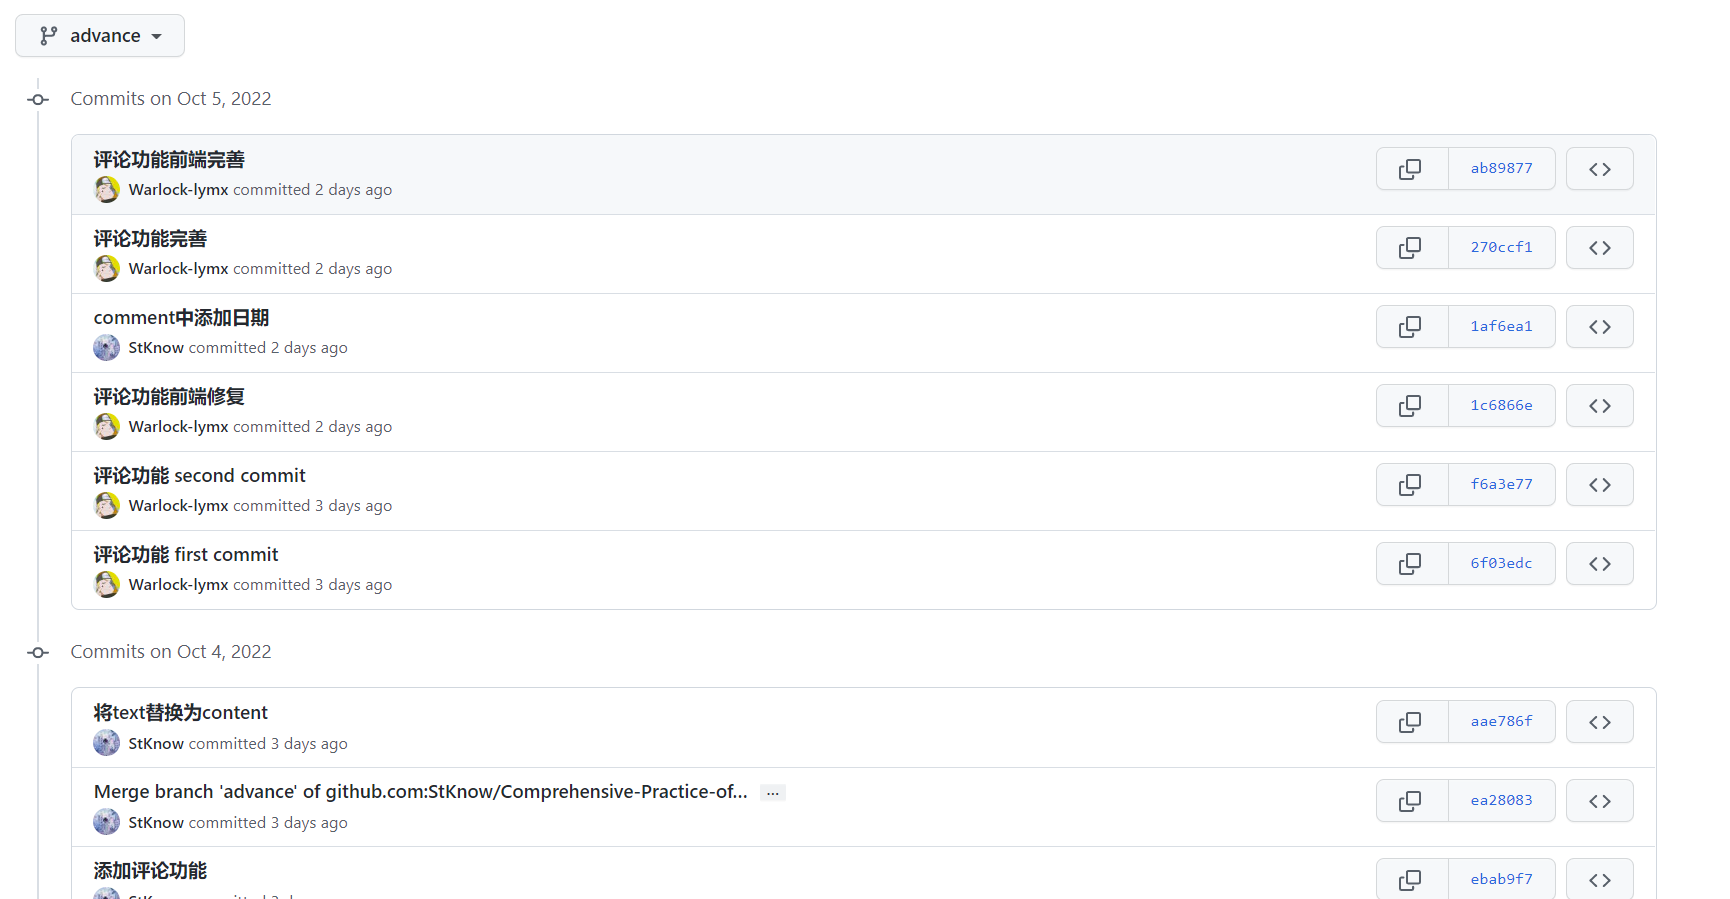
\includegraphics[width=6cm,height=4cm]{figures/6.1.5.png}\\
        \end{minipage}
    }
    \subfigure{
        \begin{minipage}[t]{0.48\linewidth}
            \centering
            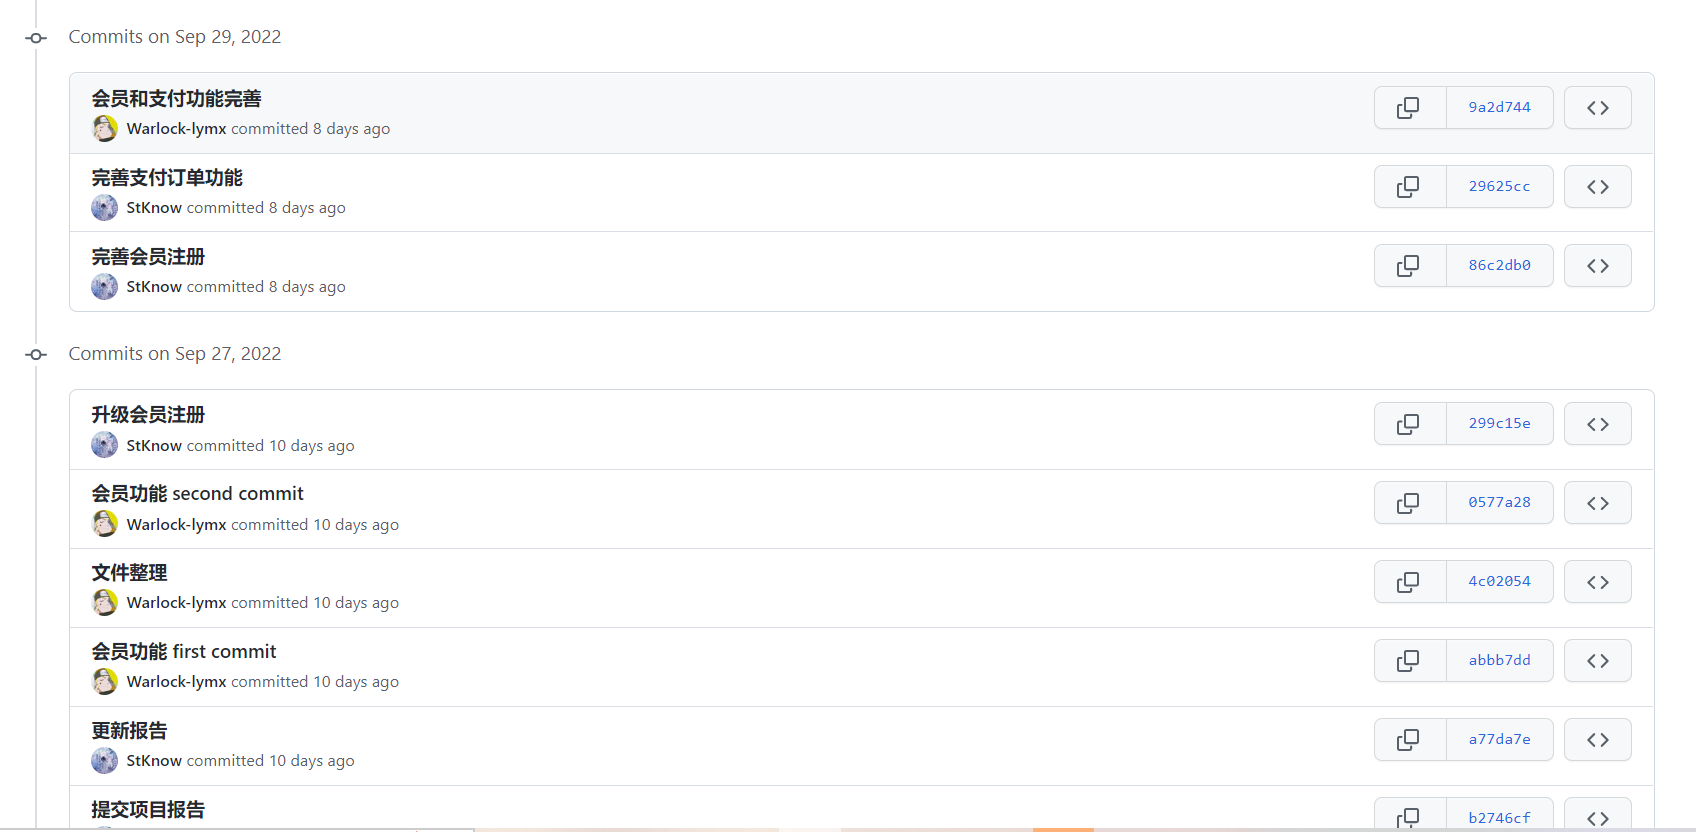
\includegraphics[width=6cm,height=4cm]{figures/6.1.6.png}\\
        \end{minipage}
    }
    \centering
    \caption{advance分支提交记录}
\end{figure}


\section{开发过程中的问题及解决方法}
问题:项目一中MySQL依赖库路径错误。

解决方法:通过错误提示发现此版本依赖库中路径少一个.cj。
\\
\par
问题:项目二前端中课件代码生成的网页显示有误。

解决方法:通过CSS中的margin属性指定外边距,从而使页面显示达到预想的效果。
\\
\par
问题:VUE框架搭建出错,版本号不对应,导致按照课件编写的网页无法正常显示页面。

解决方法:卸载VUE,重新按照视频安装对应的版本。
\\
\par
问题:router路由重定向出错,点击“去注册”按钮跳转到登录页面。

解决方法:经检查,在main.js中判断是否登录的条件出错,筛选“注册”页面未成功。将筛选条件修改正确解决问题。
\\
\par
问题:第四部分后端项目中sql语句编写错误。

解决方法:通过postman测试发现接口出现错误,通过后端报错解决问题。
\\
\par
问题:添加会员功能之后,在下订单部分下方价格部分小数点位数显示出现问题。

解决方法:通过Number(value).toFixed(2)方法限制显示的小数点位数。







